\subsection{Simple Polygons}
\label{sec:warm-up}

To get a sense of the types of problems we will encounter,
we begin by deriving a useful equation.
\begin{theorem}\label{thm:triangle}
In the plane, the sum of the interior angles of a triangle is $\pi$.
\end{theorem}
\begin{proof}
Draw a line parallel to one edge through the opposite vertex.
By alternating interior angles in the plane, the sum of the angles
in the triangle equal  a straight line.
See \figref{angles} for an illustration. 



\begin{figure}[htb]
\centering
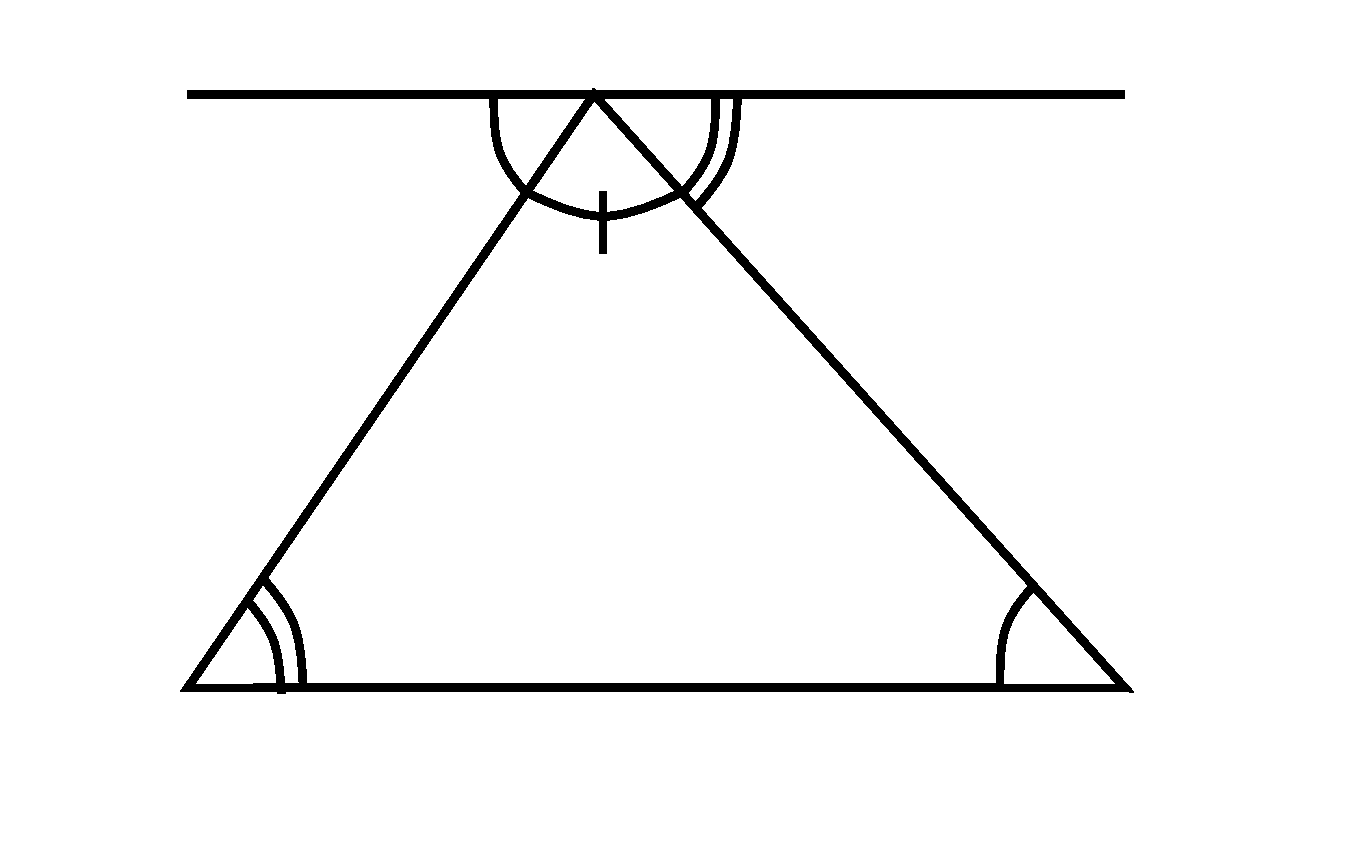
\includegraphics[width=.3\textwidth]{sec-1-and-2/interior-angles-triangle}
\caption{A proof that, in the plane, the sum of the angles of a triangle is $\pi$.}
\label{fig:angles}
\end{figure}

\end{proof}

Note the sum of the angles of a triangle does not
depend on certain properties of the  triangle, such as the orientation in the plane or
the scale factor of the triangle.


Even this simple version of the theorem is useful.
Consider any simple polygon $P$ on $n$ vertices. 
What is the sum of the interior angles of $P$?
One could measure each angle, but if $n$ is large they would eventually
get tired.
Instead, we notice that any polygon with $n$ vertices can be
triangulated with $n-2$ triangles \cite{orourke_computational_1994}.
Thus, when we traverse $P$ we go around $n-2$ triangles each contributing
$\pi$.
As a corollary to \thmref{triangle} we have
\begin{corollary}\label{cor:angles}
In the plane, any simple polygon $P$ with $n$ vertices,
the sum of the interior angles of $P$ is $(n-2)\pi$.

\end{corollary}

Now, we do not need to measure any angles to find
the sum of  the interior angles of a polygon. We can simply
count the vertices. What savings!
